\section{Предлагаемые улучшения модели BBS-Net}

В качестве базовой модели для улучшений мы взяли модель BBS-Net, представленную в \cite{BBS}.
ВПри её тренировке в качестве функции ошибки использовалась  бинарная перекрёстная энтропия,
а экстрактором признаков выступала свёрточная сеть ResNet-50\cite{ResNet}
с претренированными весами из библиотеки torchvision \footnote{\url{https://pytorch.org/vision/stable/models.html}}.

Цель наших экспериментов - улучшить метрики качества исходной модули путём использования 
других функций потерь, а также применением другого экстрактора - свёрточной сети EfficientNet B-0\cite{Efficientnet}.
Согласно анализу, представленному в \cite{Efficientnet}, в сравнении с ResNet-50 сеть EfficientNet B-0 имеет большую точность 
и в 4.9 раз меньше параметров (5.3M в EfficientNet B-0 против 26M в ResNet-50). 
Таким образом, в ходе экспериментов мы надеемся не только улучшить качество метрик, 
но и уменьшить размер модели, а также ускорить её работу.


\subsection{Функции потерь}

Для тренировки нейронных сетей используют различные алгоритмы, основанные на стохастическом градиентном спуске,
для максимизации или минимизации некоторой целевой функции. В качестве целевой функции используют различные функции потерь, 
которые нужно минимизировать. Вид этих функций зависит от типа решаемой задачи, а выбор подходящей функции напрямую влияет на 
качество обучаемой модели. 

Для решения задачи выявления самых заметных объектов на изображении 
во многих работах, в том числе и в исследуемой нами \cite{BBS}, применяется функция бинарной перекрёстной энтропии.

В результате работы модели мы ожидаем получить бинарное изображение $S \in \mathbb{R}^{W \times H}$, и $S_{i,j} \in [0,1]$, которое содержит 
выделение наиболее заметных областей и будет как можно больше соответствовать истинной карте заметности $G \in \{0,1\}^{W \times H}$
Другими словами, мы хотим классифицировать каждый пиксель на изображении и отнести его либо к группе "выделяющихся", либо "не выделяющихся". То есть,
решить задачу сегментации - классификации пикселей на изображении. Таким образом, использование бинарной перекрестной энтропии 
в качестве функции потерь вполне естественно.

Однако, за последние годы для улучшения результатов задачи сегментации изображений были предложены и другие функции потерь, подходящие для 
этой задачи \cite{Loss-Functions}. Среди них : 


\begin{itemize}
    \item Функция потерь Дайса\cite{Dice-Loss}
    \item Функция потерь Дайса Жаккара\cite{IoU-Loss}
    \item Фокальная функция потерь \cite{Focal-Loss}
\end{itemize}

Остановимся подробнее на каждой из приведённых функций.

\subsubsection{Бинарная Перекрёстная Энтропия}


Функция бинарной перекрёстной энтропии(binary cross entropy) является частным случаем функции перекрёстной энтропии - одной из самых популярных 
функций потерь для задач классификации и, как следствие, сегментации - попиксельной классификации.

Обозначим $y$ - истинную метку $\hat{p}$ - предсказанное значение.
Тогда перекрёстная энтропия \cite{CE} определяется следующим образом: 
\begin{equation}
    L_{CE} = -\sum_{i=1}^{C}y_c\log{\hat{p_c}}
\end{equation}
где $y$ - истинный класс объекта, $y_c$ - предсказанный класс, а $C$ - количество 
всех классов.

В случае предсказания только двух классов, то есть при $C=2$, 
и возможных значениях меток $y \in \{0,1\}$
перекрёстная энтропия превращается в бинарную:

\begin{equation}
    L_{CE} = -\sum_{i=1}^{2}y_c\log{\hat{y_c}} = 
    -(y\log{\hat{p}} + (1-y)\log{1-\hat{p}})
\end{equation}

\subsubsection{Dice Loss} 

Коэффициент Дайса широко используется в компьютерном зрении для оценки сходства 
между двумя изображениями. В работе \cite{Dice} была предложена адаптация коэффициента 
для использования его в качестве функции потерь. 

Пусть $y \in mathbb{R}^{N}$ - истинный вектор (который может быть выпрямленным изображением) $\hat{p} \in mathbb{R}^{N}$ - предсказанный.
Тогда функция потерь на основе коэффициента Дайса записывается в виде

\begin{equation}
    L_{DL}(y, \hat{p} ) = 1 - \frac{2y\hat{p} + 1}{y + \hat{p} + 1}
\end{equation}


\subsubsection{IoU Loss}

Коэффициент Жаккара, используется в статистике как мера сходства и различия двух множеств $A$ и $B$ \cite{IoU-Loss}:

\begin{equation}
    J(A,B) = \frac{|A \cap B|}{|A \cup B|} = \frac{|A \cap B|}{|A + B - A \cap B|}
\end{equation}

Это отношение также называют пересечением над объединением 
(Intersection over Union, IoU). В контексте задач сегментации и детекции, 
оно позволяет определить, насколько  хорошо предсказанная моделью область изображения перекрывает
область искомую.

Коэффициент Жаккара легко может быть преобразован в функцию потерь\cite{IoU-Loss-2}:

\begin{equation}
    L_{IoU} = 1- \frac{|A \cap B|}{|A \cup B|} = 1 - \frac{|A \cap B|}{|A + B - A \cap B|}
\end{equation}

\subsubsection{Focal Loss}



Фокальная функция потерь, представленная в работе \cite{Focal-Loss}, является вариацией бинарной перекрёстной энтропии.
Отличительной чертой этой функции является возможность снижать вклад простых примеров и фокусироваться на примерах, более сложных
для обучения. В частности, функция хорошо показывает себя в случае сильно несбалансированных классов.
Например, в случае когда сегментированная область гораздо меньше изображения.


\begin{equation}
    CE=\begin{cases}
        -\log{p} & \text{if }y=1\\
        -\log{1-p} & \text{if }y=0
     \end{cases}
\end{equation}

Для удобства введём новое обозначение оценочной вероятности класса:

\begin{equation}
    p_t=\begin{cases}
        p & \text{if }y=1\\
        1-p & \text{if }y=0
     \end{cases}
\end{equation}

Тогда функцию перекрёстной энтропии можно переписать как

\begin{equation}
    CE(p,y) = CE(p_t) = -\log{p_t}
\end{equation}

Фокальная функция потерь имеет вид

\begin{equation}
    FL(p_t) = -\alpha_t(1-p_t)^{\gamma}\log{p_t}
\end{equation}
 
В качестве эксперимента по улучшению существующей модели BBS-Net\cite{BBS} мы обучим модели с двумя экстракторами признаков 
(ResNet и EfficientNet) с каждой из четырёх функций потерь.
Значения гиперпараметров для фокальной функции потерь будут использованы следующие: $\alpha=0.8$ и $\gamma=2$


\subsection{Метрики Качества}

В качестве метрик качества мы будем использовать две наиболее широко используемых в задачах SOD метрики: 
среднюю абсолютную ошибку (Mean Absolute Error, MAE) и F-меру(F-measure).

Средняя абсолютная ошибка - это сумма разностей
модулей соответствующих значений пикселей предсказанного
 и истинного изображения $S$ и $G$.
\begin{equation}
    mae = \frac{1}{N}\sum_{i=1}^N|S - G|
\end{equation}
где $N = WH$ - число пикселей.


F-мера представляет собой гармонической среднее 
между точностью(precision) и полнотой(recall).

\begin{equation}
    F_1 = 2\frac{precision \times recall}{precision + recall}
\end{equation}

Точность(precision) и полнота(recall) определяются 
как отношение числа истинно-положительных решений к сумме 
числа истинно-положительных решений и ложно-положительных решений в случае 
точности(precision) или ложно-отрицательных решений в случае 
полноты(recall):

\begin{equation}
    precision = \frac{TP}{TP+FP}
\end{equation}

\begin{equation}
    recall = \frac{TP}{TP+FN}
\end{equation}

В случае оценки карты значимости, мы можем 
говорить об истинно-положительном решении 
как о присвоении пикселю значение 1 при условии, что 
пиксель на истинной карте также имеет значение 1, 
о ложно-положительном решении как о присвоении пикселю значение 1 при условии, что 
пиксель на истинной карте также имеет значение 0 
и о ложно-отрицательных решении как о присвоении пикселю значение 0 при условии, что 
пиксель на истинной карте также имеет значение 1. 

\subsection{Данные для экспериментов}

С растущим интересом к задаче RGBD-SOD, а также с распространением устройств, способных 
снимать изображением с картой глубины, за последние несколько лет появилось несколько RGB-D SOD датасетов.

Каждый датасет состоит из изображения с соответствующей ему картой глубины, а также
бинарное изображение с маской искомого выделяющегося объекта на изображении.

\begin{figure}[h]
    \centering
    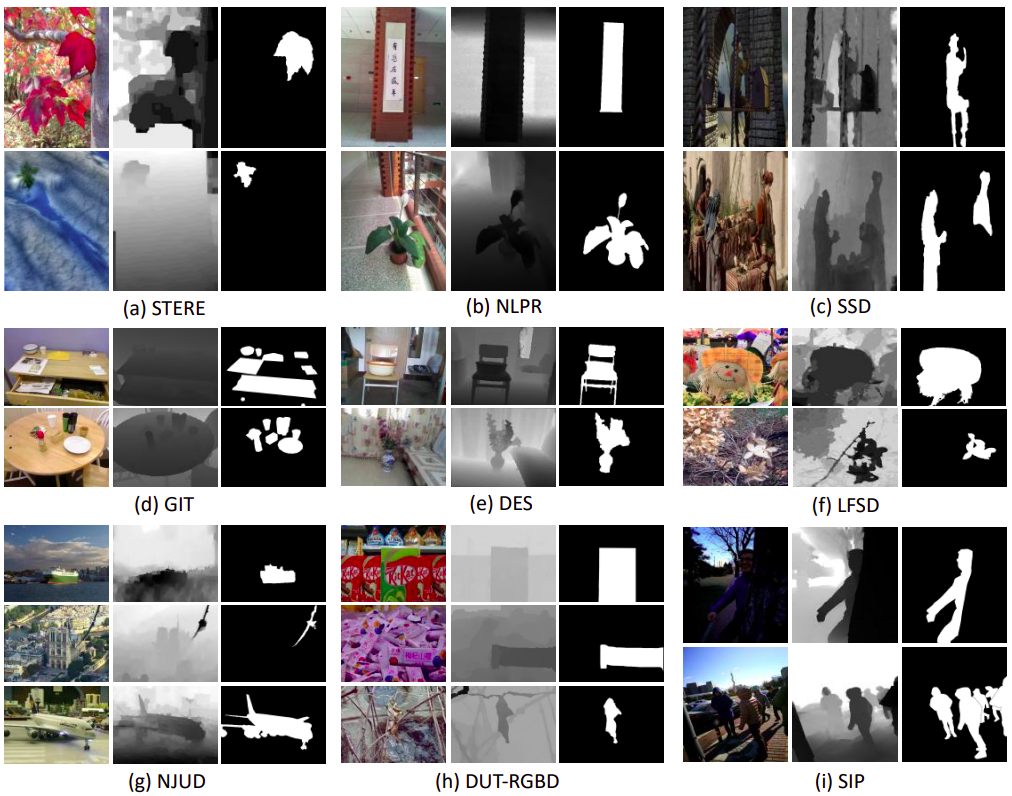
\includegraphics[width=1\textwidth]{datasets}
    \caption{Примеры изображений из различных датасетов}
    \label{fig:dataset}
\end{figure}

Ниже представлен краткий обзор существующих датасетов:
\begin{itemize}
    \item STERE \cite{STERE} - первый датасет со стереоскопическими изображениями, собранных с сайтов Flickr, NVIDIA 3D Vision Live и Stereoscopic Image Gallery
    Содержит 1000 изображений с различными разрешениями
    \item GIT \cite{GIT} - содержит 80 картинок домашней обстановки, собранных роботом.
    \item LFSD \cite{LFSD}
    \item DES \cite{DES} - небольшой датасет объёмом 135 изображений, собранных с помошью Microsoft Kinect. Разрешение изображений: 640х480.
    \item NLPR \cite{NLPR} - содержит 1000 изображений разрешением 640х480, также собранных с помошью Microsoft Kinect.
    \item NJU2K \cite{NJU2K} - самый большой датасет, содержащий 1985 изображений с разными разрешениями, собранных из интернета, 3D фильмов и снятых на стерео камеру Fuji W3.
    \item SSD \cite{SSD} - содержит 80 картинок с высоким разрешением 960х1080, собранных из 3D фильмов.
    \item DUT-RGBD \cite{DUT} - содержит 1200 изображений со сложными для модели факторами, например: однотипный передний план или похожие передние и задние планы
    \item SIP \cite{Rethinking-RGBD} - содержит 1000 изображений с разрешением 992х744, снятых на смартфон
\end{itemize}


\begin{center}
    \begin{table}
        \begin{tabular}{|c|c|c|c|c|} 
            \hline
            Датасет & Год & Размер & Разрешение\\
            \hline
            \hline
            STERE\cite{STERE} & 2012 & 1000 & $[251 \sim 1200] \times [222 \sim 900]$ \\
            \hline
            GIT\cite{GIT} & 2013 & 80 & $640 \times 480$ \\
            \hline
            LFSD\cite{LFSD} & 2014 & 100 & $360 \times 360$ \\
            \hline
            DES\cite{DES} & 2014 & 135 & $640 \times 480$  \\
            \hline
            NLPR\cite{NLPR} & 2014 & 1000 &  $640 \times 480$ \\
            \hline
            NJU2K\cite{NJU2K} & 2014 & 1985 & $[231 \sim 1213] \times [274 \sim 828]$\\
            \hline
            SSD\cite{SSD} & 2017 & 80 & $960 \times 1080$\\
            \hline
            SIP\cite{Rethinking-RGBD} & 2020 & 929 &  $992 \times 744$\\
            \hline
        \end{tabular}
    \caption{Эксперименты}
    \label{tab:datasets}
    \end{table}
\end{center}

В таблице \ref{tab:datasets} представлены характеристики датасетов, год выхода, количество изображений и их разрешение.
Примеры изображений из различных датасетов представлен на схеме \ref{fig:dataset}


Каждую модель мы будем обучать и валидировать на датасете NJU2K. Остальные датасеты будут тестовыми. На них мы будем
запускать обученные модели и считать метрики качества.

\subsection{Описание экспериментов}

Имплементация моделей, код для тренировки и валидации, функций потерь и метрик качества были написаны на языке Python 3.8
с использованием фреймворка для глубокого обучения Pytorch 1.8.0\cite{Pytorch}.


В работе была использована оригинальная имплементация модели от авторов статьи \cite{BBS}, 
которая доступна на GitHub \footnote{\url{https://github.com/zyjwuyan/BBS-Net}}.
На её основе была написана модель BBS-Net, которая в качестве свёрточной сети для извлечения признаков
использовала сеть EfficientNet-B0 \cite{Efficientnet} с весами, предобученными на датасете ImageNet
\footnote{\url{https://github.com/lukemelas/EfficientNet-PyTorch}}.


Все модели тренировались и валидировались на датасете NJU2K предварительно разделённым на NJU2K\_TRAIN для тренировки, 
который содержит 1485 изображений, и NJU2K\_TRAIN для промежуточной валидации, содержащий 500 изображений.
Каждая тренировка состояла из 150 эпох с размером пакета(batch size) равным 10. В конце каждой эпохи запускалась валидация: рассчитывалось среднее
значение функции потерь и средней абсолютной ошибки(MAE), минимальное значение которой сохраняется и обновляется во время
всего процесса тренировки. В случае обновления значения - текущее состояние модели сохраняется и помечается наилучшим в смысле качества обучения.
В результате тренировки мы получаем модель, которая показывает наименьшую ошибку на валидационном датасете. Такая стратегия используется для того,
чтобы избежать переобучения под тренировочный датасет. 
Для тренировки модели использовался стандартный оптимизатор Adam\cite{Adam}. Начальное значение параметра скорости обучения(learning rate) 
равно 0.0001. Каждые 60 эпох значение уменьшалось в 10 раз \ref{fig:lr}. Такой подход был предложен в оригинальной работе \cite{BBS}.


\begin{figure}[h]
    \centering
    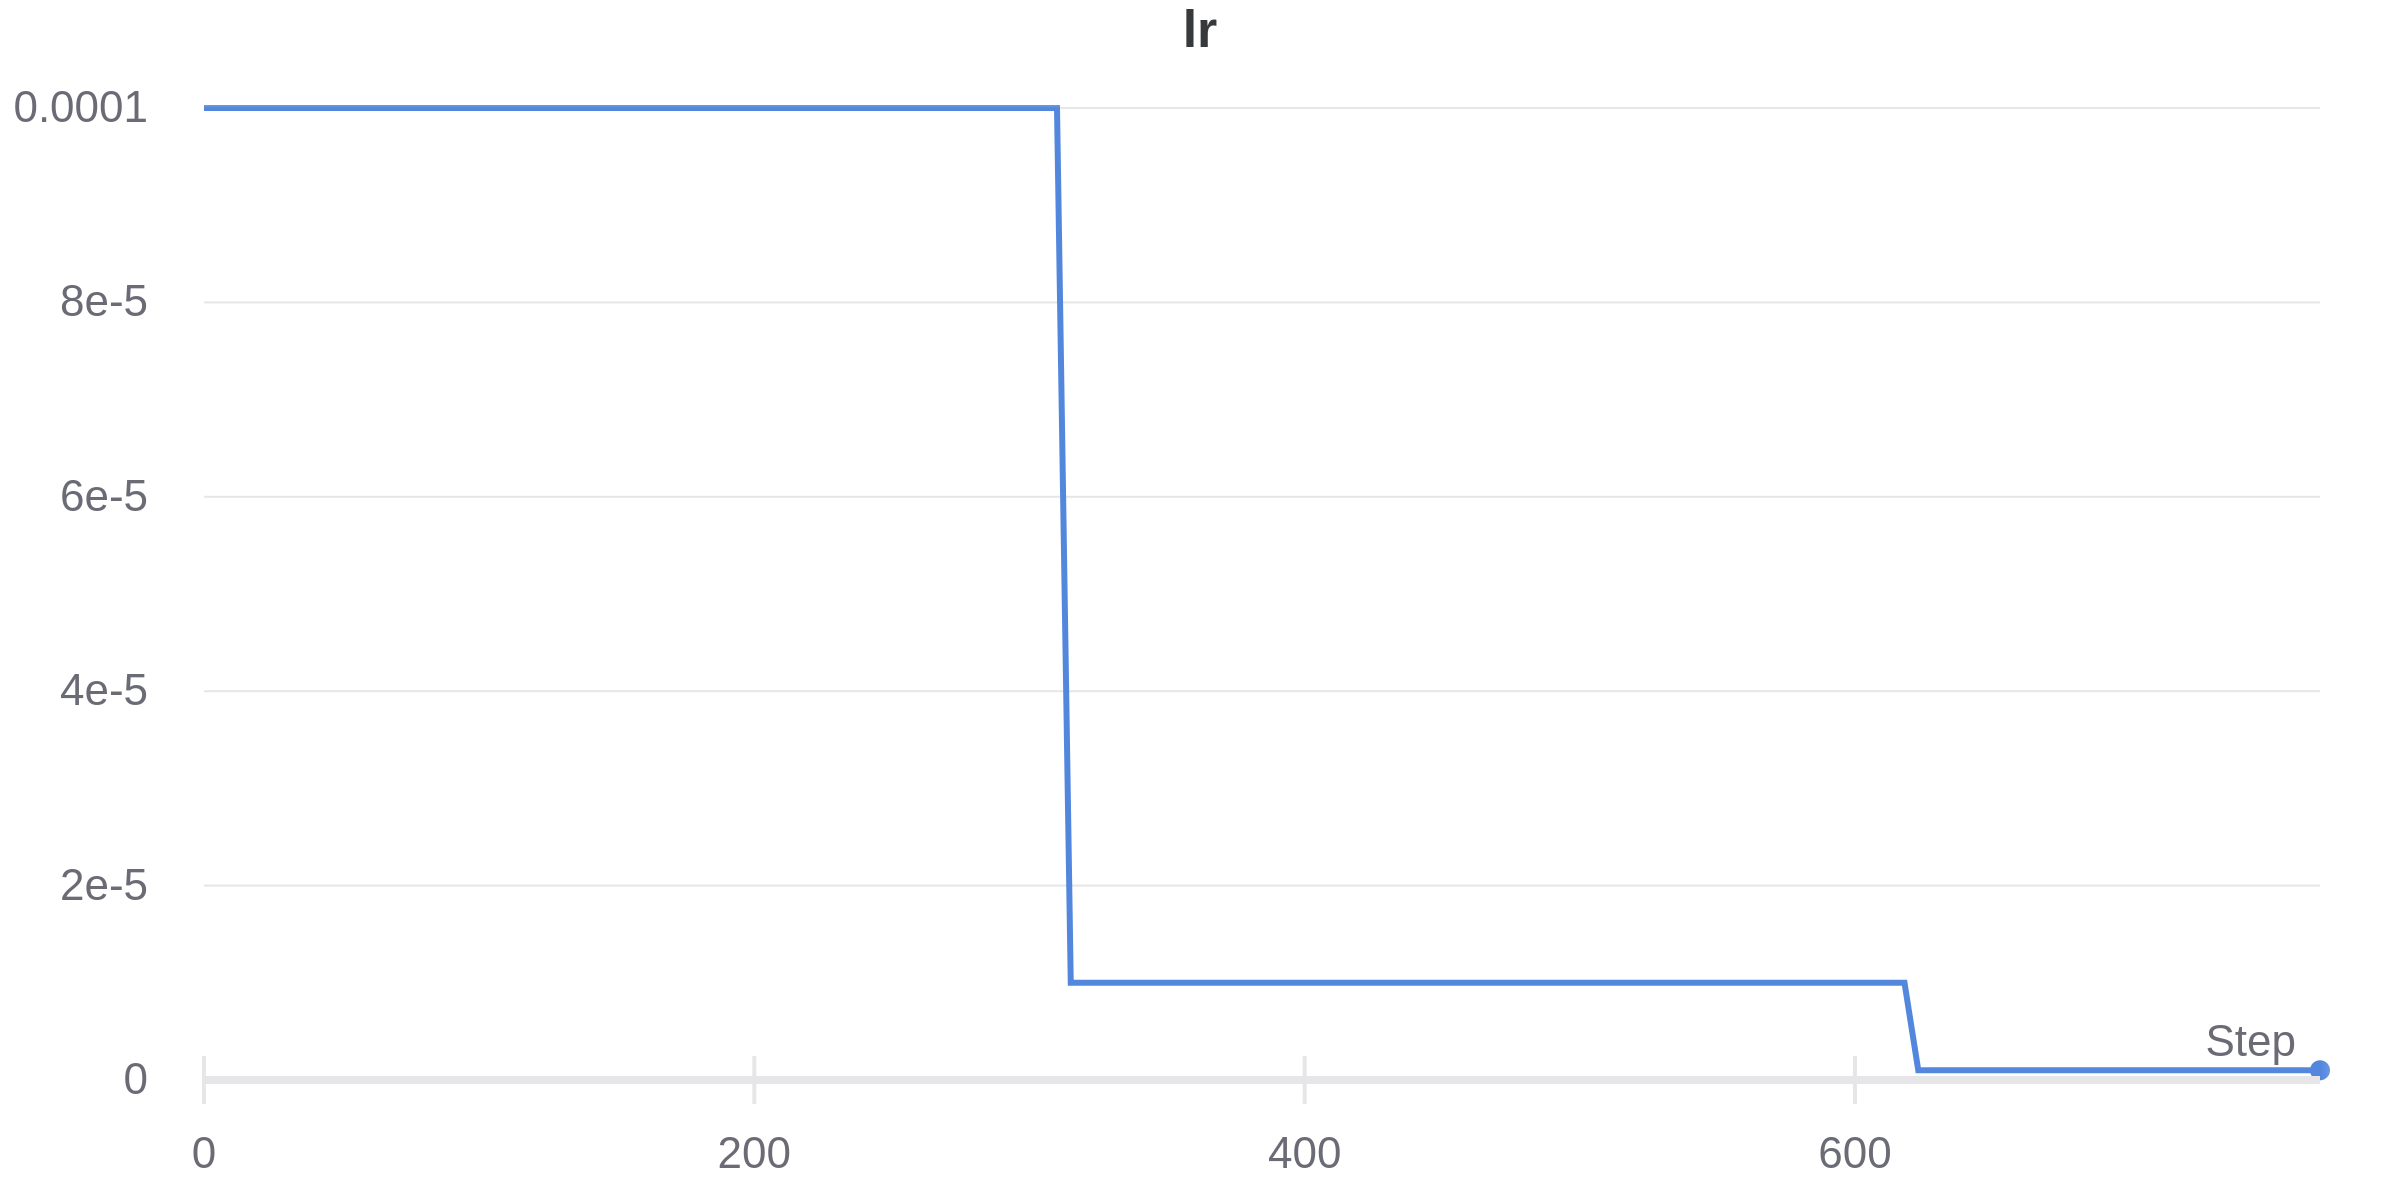
\includegraphics[width=0.6\textwidth]{lr}
    \caption{Изменения скорости обучения при тренировке}
    \label{fig:lr}
\end{figure}

На вход модели подаются RGB изображение и карта глубины с разрешением 352х352 как на этапе тренировки, там и на этапе расчёта тестовых метрик.
Так как изображения в датасетах имеют разные размеры, перед передачей применяется изменение размера, а также, на этапе тренировки, некоторые приёмы аугментации 
изображения: поворот, масштабирование, кроп. Все преобразования выполняются через стандартные классы для работы с данными в Pytorch: Dataset и DataLoader
\footnote{\url{https://pytorch.org/docs/stable/data.html}}
Все эксперименты проводились на платформе Google Colab\footnote{\url{https://colab.research.google.com/notebooks/intro.ipynb}}
с GPU Tesla P100-PCIE-16GB.


\begin{center}
    \begin{table}
        \begin{tabular}{ |c c|c|c|c|c|c|c|c|c| } 
            \hline
            \multirow{2}{*}{\rotatebox[origin=c]{90}{Датасет}} & \multirow{2}{*}{Метрика} & \multicolumn{4}{ |c| }{ResNet} & \multicolumn{4}{ |c| }{EfficientNet} \\
            \cline{3-10}
            & & BCE & focal & dice & IoU & BCE & focal & dice & IoU\\
            \hline
            \multirow{2}{*}{\rotatebox[origin=c]{90}{NJU2K}} & mae $\downarrow$ &0,033&0,06&0,031&0,032&0,035&0.057&0,031&\textbf{0,030} \\
            & f1  $\uparrow$ &0,909&0,832&\textbf{0,920}&0,915&0,901&0.842&0,916&0,918\\
            \multirow{2}{*}{\rotatebox[origin=c]{90}{NLPR}} & mae $\downarrow$ &0,041&0,065&0,040&0,037&0,040&0.059&0,039&\textbf{0,034} \\
            & f1  $\uparrow$ &0,840&0,734&0,856&0,858&0,838&0.756&0,846&\textbf{0,865}\\
            \multirow{2}{*}{\rotatebox[origin=c]{90}{DES}} & mae $\downarrow$ &0,019&0,041&0,017&\textbf{0,015}&0,019&0.039&0,016&0,016\\
            & f1  $\uparrow$ &0,916&0,819&0,930&\textbf{0,939}&0,918&0.822&0,933&0,929\\
            \multirow{2}{*}{\rotatebox[origin=c]{90}{SSD}} & mae $\downarrow$ &0,046&0,073&0,044&0,046&0,047&0.068&0,043&\textbf{0,041} \\
            & f1  $\uparrow$ &0,841&0.777&0,855&0,851&0,844&0.777&0,860&\textbf{0,863}\\
            \multirow{2}{*}{\rotatebox[origin=c]{90}{STERE}} & mae $\downarrow$ &0,039&0,066&0,037&\textbf{0,035}&0,039&0.063&0,037&0,036 \\
            & f1  $\uparrow$ &0,888&0,817&0,898&\textbf{0,905}&0,891&0.824&0,899&0,903\\   
            \multirow{2}{*}{\rotatebox[origin=c]{90}{LFSD}} & mae $\downarrow$ &0,077&0,104&\textbf{0,066}&0,072&0,074&0.102&0,082&0,072\\
            & f1  $\uparrow$ &0,843&0,782&\textbf{0,862}&0,859&0,843&0.789&0,834&0,851\\  
            \multirow{2}{*}{\rotatebox[origin=c]{90}{SIP}} & mae $\downarrow$ &0,047&0,07&0,045&0,044&0,047&0.069&0,051&\textbf{0,042}\\
            & f1  $\uparrow$ &0,867&0,789&0,877&0,88&0,87&0.809&0,859&\textbf{0,884}\\  
            \multirow{2}{*}{\rotatebox[origin=c]{90}{DUT}} & mae $\downarrow$ &0,121&0,145&0,116&0,121&0,112&0.122&\textbf{0,105}&0,14\\
            & f1  $\uparrow$ &0,592&0,574&0,67&0,597&0,65&0.639&0,707&\textbf{0,728}\\  
            \hline
        \end{tabular}
    \caption{Эксперименты}
    \label{tab:experiments}
    \end{table}
\end{center}

Результаты эксперимента описаны в таблице \ref{tab:experiments}. 
Видно, что специализированные функции потерь для задачи сегментации
показали свою эффективность. Лучшие результаты метрик на всех исследованных
датасетах показали модели, обученные либо с функцией потерь Дайса, либо с функцией потерь Жаккарта
При этом, модели, обученные с функцией потерь Жаккарта лучшие по обеим метрикам
на датасетах NLPR, DES, SSD, STERE, SIP. Модели, обученные с функцией потерь Дайса 
по обеим метрикам лучшие только на датасете LFSD.

Эксперимент с заменой свёрточной сети для извлечения признаков с ResNet на EfficientNet b-0 
так же оказался удачным. На половине датасетов модели на основе EfficientNet b-0 показали 
лучшие результаты по обеим метрикам и на датасете NJU2K - лучший результат по метрике $mae$.

При этом, новые модели опережают результаты бейзлайна.


\subsection{Инференс моделей}

Кроме вычисления метрик на разных датасетах, были проведены эксперименты по измерению
инфреренса(?) моделей BBS-Net, основанных на ResNet-50 и EffecientNet-B0. 
Для экспермиента был сгенерирован два искусственный пакета, в каждом по единственной матрице, размерности 
$3 \times 352 \times 352$ и $1 \times 352 \times 352$, эмулирующих RGB изображение и карту глубины.
Время работы модели измерялось на GPU Tesla P100-PCIE-16GB с помощью пакета Pytorch.cuda\footnote{\url{https://pytorch.org/docs/stable/cuda.html}}
Результаты замеров представлены в таблице \ref{tab:inference}

\begin{center}
    \begin{table}
        \begin{tabular}{ |c|c|c| } 
            \hline
            Экстрактор признаков & Среднее время(мс) & Стандартное отклонение(мс) \\
            \hline
            EfficientNet-B0&51.22&1.59\\
            \hline
            ResNet&40.36&0.55 \\
            \hline
        \end{tabular}
        \caption{Измерение инференса}
        \label{tab:inference}
        \end{table}
    \end{center}

Получается, что несмотря на большее число параметров, модель BBS-Net, основанная на ResNet-50 работает быстрее, чем модель, использующая EfficientNet-B0 в качестве 
экстрактора признаков.  